\chapter{Introduction}
\label{ch:Introduction}
In 2015 195 countries 

\begin{itemize}
    \item Have you ever heard of climate change?
    \item Coal bad, change to renewable...
    \item The "Gesetz zur Reduzierung und zur Beendigung der Kohleverstromung" Act aims to phase out coal-fired power generation no later than 2038
    \item Iron good option
    \item Iron is an interesting recyclable fuel due to the fact that it is
widely available, has a low cost, is non-toxic, and can be recycled
without CO2 emissions using today’s technology.
    \item Diagram: Power consumption and power production
    \item With \url{https://climate.copernicus.eu/esotc/2022/clouds-and-sunshine-duration} "As with cloud cover, the large positive anomaly for 2022 is consistent with the pronounced trend toward longer sunshine duration observed over the past four decades."
    \item "The world will not be able cope with climate change without a global energy transition. The burning of fossil fuels for power generation is the single most important cause of climate change."  \url{https://www.bmz.de/en/issues/climate-change-and-development/energy-and-climate}
    \item Recognizing that without deep emissions cuts from heavy industry and advances in clean technology
industries (including renewable energy technologies, energy storage, energy efficiency, circular
production, and sustainable mining) – collectively referred to as ‘green industrialization’ – global
carbon emissions reduction goals, in line with the Paris Agreement, cannot be met,
\url{https://cop30.br/en/news-about-cop30/cop30-documents/cop30_belem-declaration-on-global-green-industrialization_final-4.pdf/@@download/file}
\item Paris Agreement Article 2a) Holding the increase in the global average temperature to well below
2°C above pre-industrial levels and pursuing efforts to limit the temperature
increase to 1.5°C above pre-industrial levels, recognizing that this would
significantly reduce the risks and impacts of climate change;
\item Figure ES.1 from \url{https://wedocs.unep.org/bitstream/handle/20.500.11822/46404/EGR2024.pdf?sequence=3&isAllowed=y} 25\% of all emissions due to power generation, largest is energy production
\item \url{https://de.statista.com/statistik/daten/studie/37595/umfrage/anteil-einzelner-sektoren-an-den-co2-emissionen-in-deutschland/} CO2 emissions in Germany in 2024 31.3\% due to the energy sector
\item Both the CPS and the STEPS project electricity demand reaching essentially the
same level in 2035, around 37 800 terawatt-hours (TWh). This represents an increase of 40\%
from today’s level and an acceleration of the pace of growth compared to the past decade. (Section 1.1) \url{https://iea.blob.core.windows.net/assets/9228d782-4207-4648-9c75-e6bb908cdb90/WorldEnergyOutlook2025.pdf}
\item Out of all of the metals identified as possible energy carriers, silicon, aluminum, and iron are the 2nd, 3rd, and 4th most abundant elements in the Earth’s crust, respectively [73]
\item Zur Einspeicherung von Energie
wird Eisenoxid elektrochemisch mit erneuerbarem Strom oder thermochemisch mit grünem Wasser-
stoff zu Eisen reduziert. Die thermochemische Umsetzung von Eisenoxiden bietet sich aufgrund des
fortgeschrittenen Technologiestands durch die Forschung auf dem Gebiet der nachhaltigen Produk-
tion von Stahl an. Die Ausspeicherung der Energie erfolgt durch die Oxidation von Eisen mithilfe
von Luftsauerstoff.

    \item \ldots
    \item Space to start MPPIC
    \item  Particle-particle interactions are represented by models which utilise mean values calculated on the Eulerian mesh.
    \item Collisional damping models are included to represent the mean loss in kinetic energy which occurs as particles collide. The code includes a relaxation model which uses a time-scale to calculate the rate of interaction of a particle’s momentum with that of the mean field. This helps produce physically realistic scattering behaviour, but can have a detrimental affect on the packing modelling.
    \item Collisional isotropy models represent the scattering which occurs as a result of particle collisions. The code includes a stochastic model which uses a time-scale to calculate the probability of a particle undergoing a collision, which randomises its velocity. Momentum and energy are explicitly conserved as a second step. This approach also helps to spread the particles uniformly across cells, which improves the quality of computed averages.
    \item MPPIC has stability issues. Mostly this is when the parcels are too large relative to the cells, meaning a reliable average cannot be computed.
    \item Removing drag and isotropy will cause more scattering. Both act to reduce relative velocities within the system. Both will, in all likelihood, be necessary to get a physical solution. Damping, too, is important, as it is the only mechanism by which the sub-grid collision modelling dissipates energy.
    \item The Multiphase Particle in Cell (MP-PIC) is an Eulerian-Lagrangian numerical method that resolves the particle-particle interactions using the averages mapped from the Lagrangian parcels onto the Eulerian mesh.
    \item ...
    \item An advantage of the fluidized bed reactor is that due to the raping mixing near isothermal conditions are reached throughout the reactor. 
Constant mixing, due to bubbles being formed and rising to and breaking the surface, improves the contact of solid and gas and amplifies heat and mass transfer. 

\end{itemize}
\begin{figure}
    \centering
    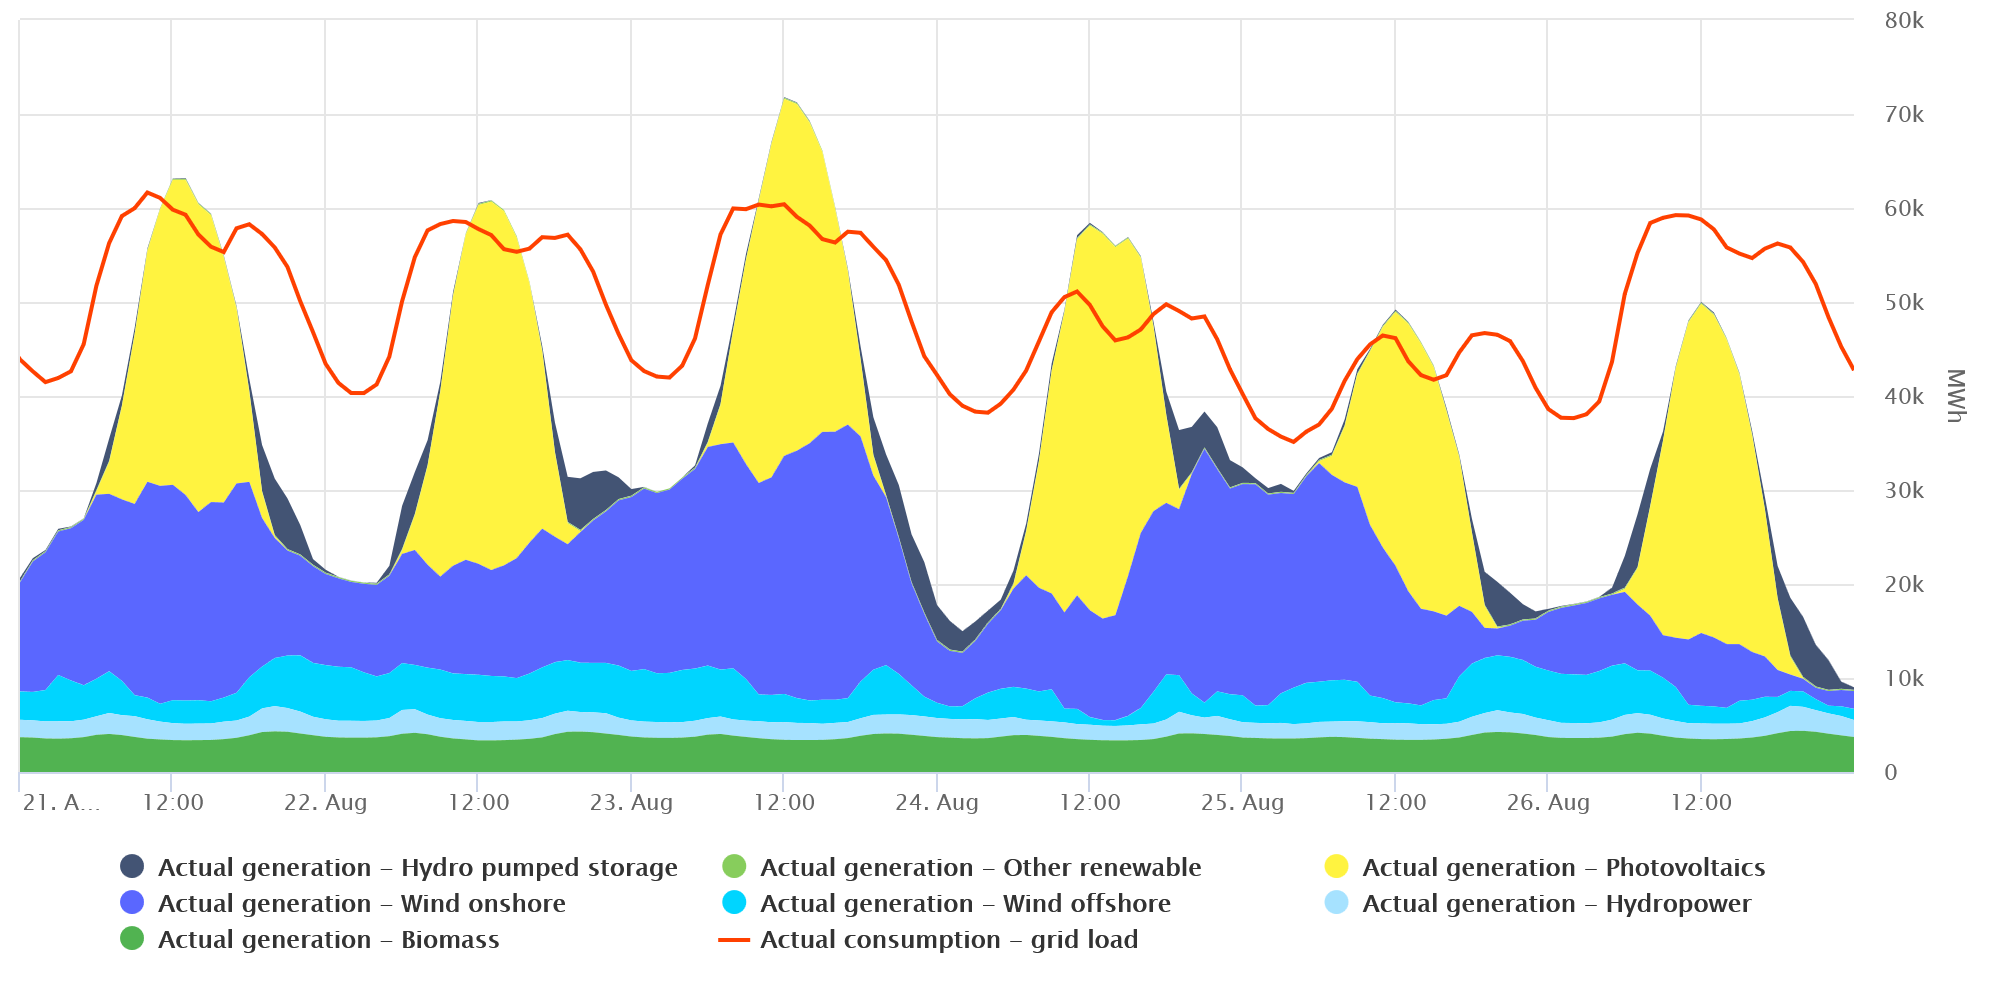
\includegraphics[width=0.9\linewidth]{sections/images/SMARD_diagram___ 20240821_20240826.png}
    \caption[Data source: SMARD]{Data source: "Bundesnetzagentur | SMARD.de" \protect\footnotemark}
    \label{fig:placeholder}
\end{figure}

%\footnotetext{\url{https://www.smard.de/en/marktdaten?marketDataAttributes=%7B%22resolution%22:%22hour%22,%22from%22:1724197320620,%22to%22:1724715720619,%22moduleIds%22:%5B1001226,1001225,1004067,1004068,1001228,1004070,5000410,1004066%5D,%22selectedCategory%22:null,%22activeChart%22:true,%22style%22:%22color%22,%22categoriesModuleOrder%22:%7B%7D,%22region%22:%22DE%22%7D}}
\footnotetext{\footurl}









% \chapter{Introduction}
% \label{ch:Introduction}

% \section{The Global Energy Challenge}

% The mitigating of climate change stands as the defining challenge of the 21st century. In 2015, 195 nations adopted the Paris Agreement, legally binding themselves to Article 2a: holding the increase in the global average temperature to well below 2°C above pre-industrial levels and pursuing efforts to limit the temperature increase to 1.5°C. Achieving these targets requires a fundamental restructuring of the global energy landscape, as the burning of fossil fuels for power generation remains the single most significant driver of climate change. According to the United Nations Environment Programme (UNEP), the energy sector accounts for approximately 25\% of all global emissions, a figure that rises to 31.3\% in Germany specifically.



% Recognizing this, legislative frameworks such as Germany's "Gesetz zur Reduzierung und zur Beendigung der Kohleverstromung" (Coal Exit Act) have mandated the phase-out of coal-fired power generation no later than 2038. However, this transition is complicated by a simultaneous surge in demand. The International Energy Agency (IEA) projects that global electricity demand will reach approximately 37,800 TWh by 2035—an increase of 40\% from current levels.

% \section{The Intermittency Problem and Iron as an Energy Carrier}

% The shift toward renewable energy sources, while necessary, introduces the challenge of volatility. Unlike fossil fuel plants, solar and wind power generation are inextricably linked to weather conditions. Data from the Copernicus Climate Change Service highlights that while sunshine duration is trending upwards, it remains variable. Consequently, there are periods where renewable generation cannot meet the baseload demand.

% \begin{figure}[h!]
%     \centering
%     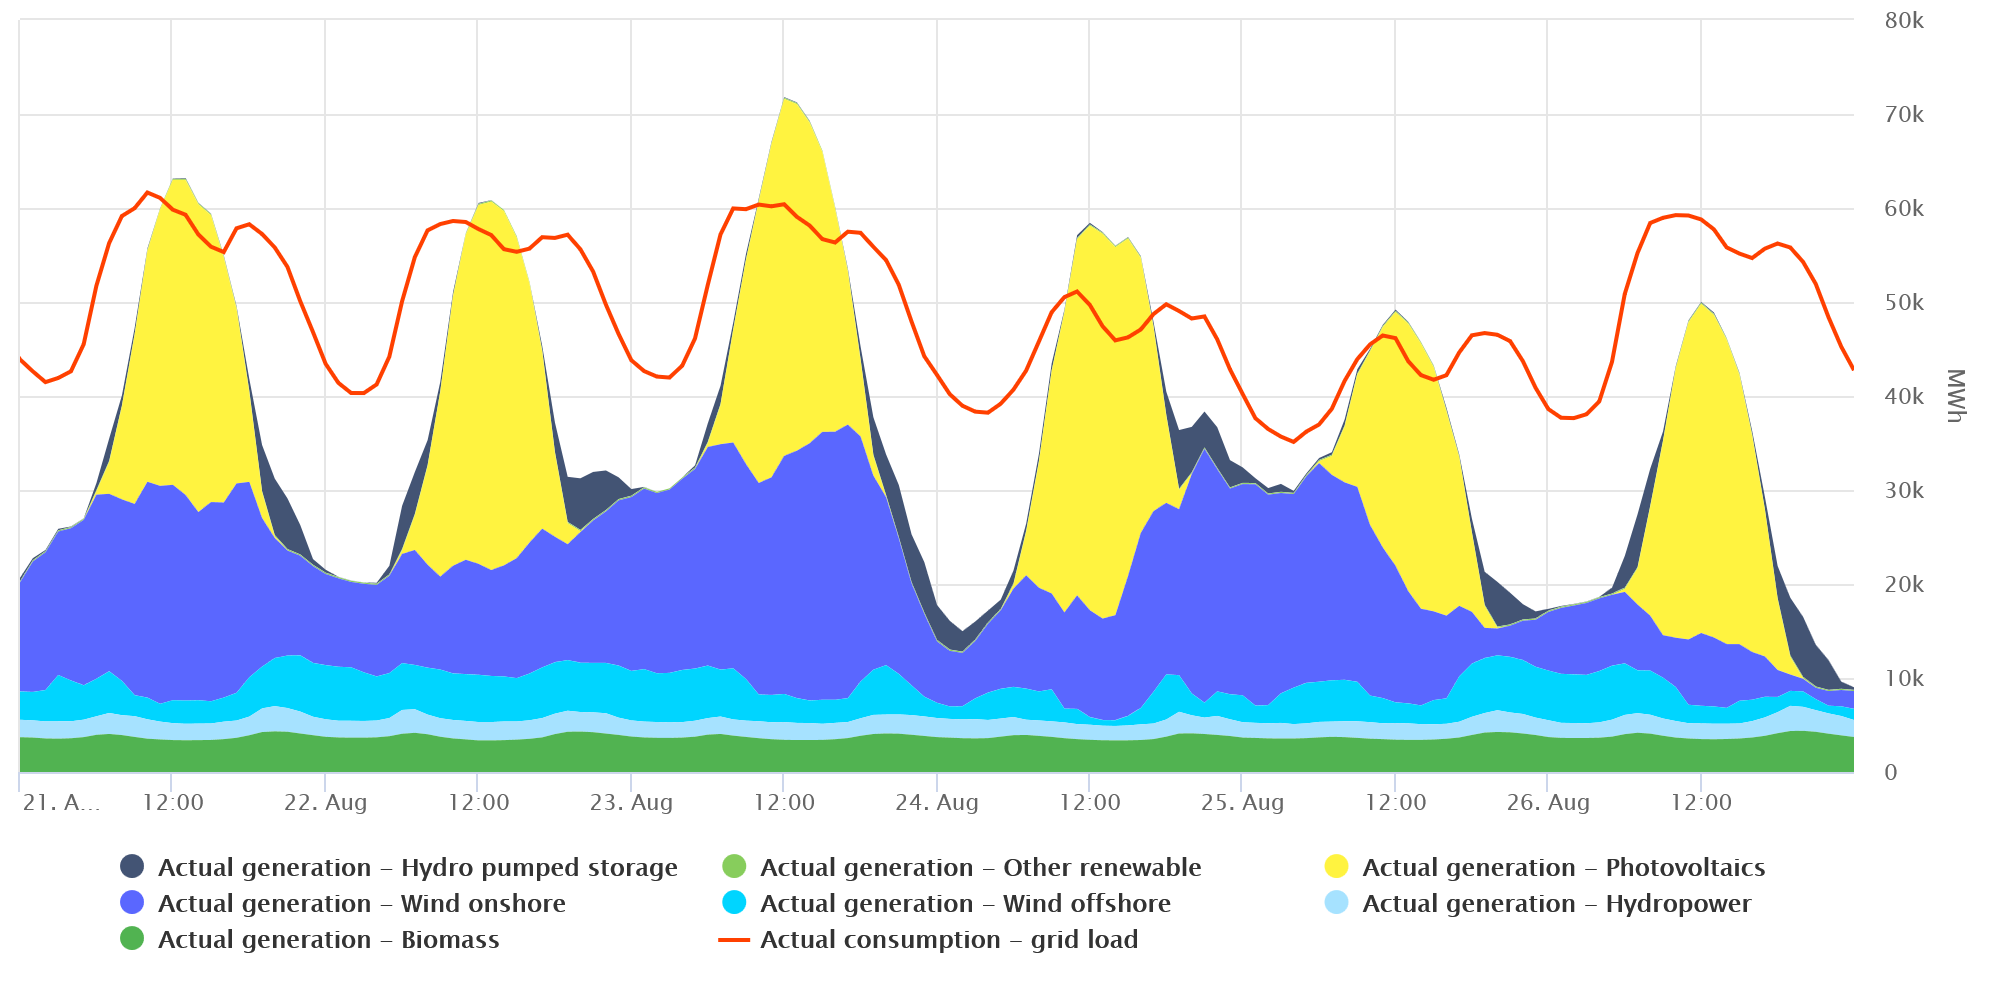
\includegraphics[width=0.9\linewidth]{sections/images/SMARD_diagram___ 20240821_20240826.png}
%     \caption[Power generation vs. Consumption]{Electricity consumption versus generation in Germany (August 2024). The discrepancy highlights the need for dispatchable energy storage. Data source: Bundesnetzagentur | SMARD.de \protect\footnotemark}
%     \label{fig:smard_data}
% \end{figure}
% \footnotetext{\url{https://www.smard.de/en}}

% To bridge the gap between volatile production and rising demand, large-scale, carbon-free energy storage is required. Metal fuels have emerged as a promising solution. Specifically, the iron/iron-oxide cycle offers a circular economy approach to energy storage. In this cycle, energy is stored by reducing iron oxide to metallic iron (using green hydrogen or renewable electricity) and released by oxidizing the iron with air.



% Iron is uniquely suited for this role for several reasons:
% \begin{itemize}
%     \item \textbf{Abundance:} It is the fourth most abundant element in the Earth's crust, ensuring wide availability.
%     \item \textbf{Safety and Cost:} Iron is non-toxic, low-cost, and possesses a high energy density.
%     \item \textbf{Technological Maturity:} The thermochemical reduction of iron oxide can leverage existing knowledge and infrastructure from the sustainable steel production industry.
% \end{itemize}

% \section{Process Technology: The Fluidized Bed Reactor}

% The reduction of iron oxide for energy storage is optimally conducted in a Fluidized Bed Reactor (FBR). In an FBR, solid particles are placed on a porous plate and suspended by an upward-flowing gas stream. This fluidization transforms the granular bed into a state behaving like a fluid, facilitating rapid mixing.



% This regime offers distinct advantages for the reduction process. The constant formation and breaking of bubbles amplifies heat and mass transfer between the gas and solid phases. Consequently, near-isothermal conditions can be maintained throughout the reactor, which is critical for consistent chemical reaction rates.

% \section{Computational Methodology: The MP-PIC Method}

% Optimizing FBRs for iron reduction requires a detailed understanding of the complex multiphase granular flow. To simulate this, this thesis utilizes \texttt{MPPICFoam}, a solver based on the Multiphase Particle-in-Cell (MP-PIC) method within the OpenFOAM framework.

% The MP-PIC method is a hybrid Eulerian-Lagrangian approach. Unlike Discrete Element Methods (DEM) which explicitly resolve every collision—a computationally prohibitive task for industrial scales—MP-PIC resolves particle-particle interactions using mean values mapped from Lagrangian parcels onto an Eulerian mesh.

% Key components of this modeling approach include:
% \begin{itemize}
%     \item \textbf{Collisional Damping:} Models the mean loss of kinetic energy during collisions. This is the primary mechanism for dissipating energy in the sub-grid modeling.
%     \item \textbf{Collisional Isotropy:} A stochastic model that represents scattering. It randomizes particle velocity based on a calculated time-scale, ensuring physically realistic scattering behavior and uniform particle distribution, which improves the quality of computed averages.
%     \item \textbf{Stability Considerations:} The method can exhibit stability issues, particularly when parcel sizes are large relative to the grid cells, compromising the reliability of the Eulerian averages.
% \end{itemize}

% This thesis aims to investigate the feasibility and optimization of the iron oxide reduction process within an FBR using these computational tools, contributing to the development of a sustainable, carbon-free energy cycle.










